\documentclass[spanish, fleqn]{article}
\usepackage[spanish]{babel}
\usepackage[utf8]{inputenc}
\usepackage{amsmath}
\usepackage{amsfonts,txfonts}
\usepackage{mathrsfs}
\usepackage{graphicx}
\usepackage[colorlinks, urlcolor=blue]{hyperref}
\usepackage{fourier}
\usepackage[top = 2.5cm, bottom = 2cm, left = 2cm, right = 2cm]{geometry}

% Default fixed font does not support bold face
\DeclareFixedFont{\ttb}{T1}{txtt}{bx}{n}{12} % for bold
\DeclareFixedFont{\ttm}{T1}{txtt}{m}{n}{12}  % for normal

% Custom colors
\usepackage{color}
\definecolor{deepblue}{rgb}{0,0,0.5}
\definecolor{deepred}{rgb}{0.6,0,0}
\definecolor{deepgreen}{rgb}{0,0.5,0}

\usepackage{listings}

% Python style for highlighting
\newcommand\pythonstyle{\lstset{
language=Python,
basicstyle=\ttm,
otherkeywords={self},             % Add keywords here
keywordstyle=\ttb\color{deepblue},
emph={MyClass,__init__,np},          % Custom highlighting
emphstyle=\ttb\color{deepgreen},    % Custom highlighting style
stringstyle=\color{deepgreen},
frame=tb,                         % Any extra options here
showstringspaces=false            % 
}}


% Python environment
\lstnewenvironment{python}[1][]
{
\pythonstyle
\lstset{#1}
}
{}

% Python for external files
\newcommand\pythonexternal[2][]{{
\pythonstyle
\lstinputlisting[#1]{#2}}}

% Python for inline
\newcommand\pythoninline[1]{{\pythonstyle\lstinline!#1!}}


\title{Tarea N°1 \\INF393: Máquinas de Aprendizaje}
\author{Martín Villanueva A.}
\date{3 de noviembre 2015}

\begin{document}
\maketitle

\thispagestyle{empty}

\section*{Introducción}

En es primera tarea, se tiene como objetivo la implementación y testeo de algoritmos para regresión lineal y regresión logística. En ambos casos la busqueda de  los mejores parámetros del modelo se realiza por medio de 	\textit{Gradiente Descendente} (batch y online) y \textit{Newton-Raphson}. Para la correcta selección de los \textit{hiperparámetros} se realiza 5-fold crossvalidation, intentando de este modo que los modelos resultantes no caigan en problemas de \textit{overfitting}.

\section*{Parte 1 - Regresión Lineal}

\begin{enumerate}
\item 

\subsection*{a) Gradiente Descendente Batch}

\subsubsection*{Raw data}

\begin{figure}[!htpb]
\centering
 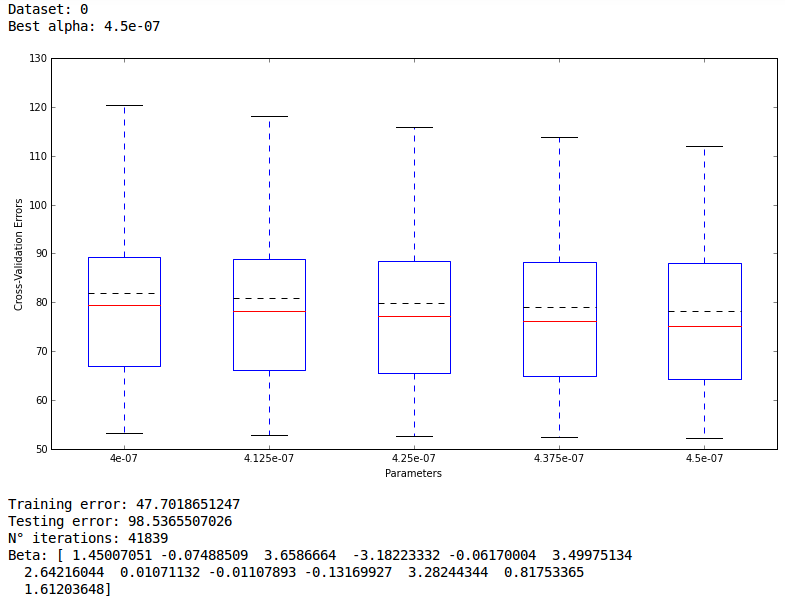
\includegraphics[scale=0.45]{gd_batch_raw0.png}
 \caption{Gradiente Descendente Batch - Raw data - dataset 0}
\end{figure}

\begin{figure}[!htpb]
\centering
 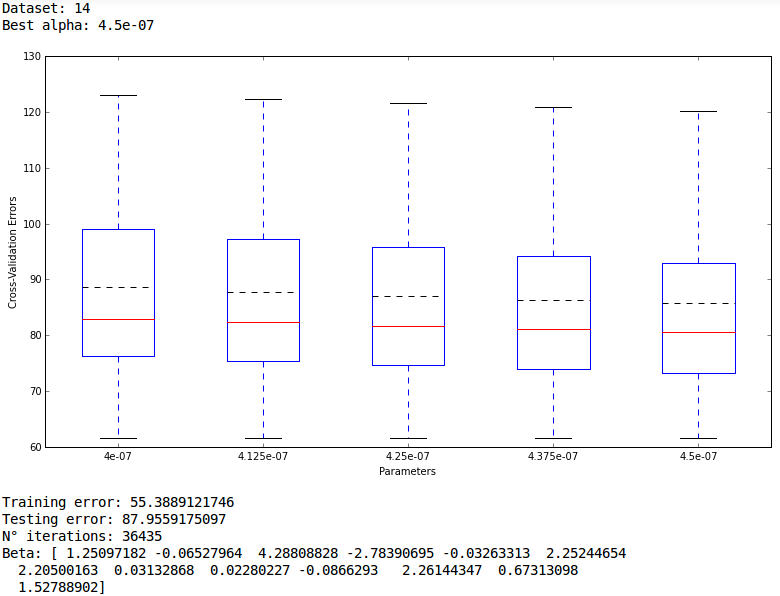
\includegraphics[scale=0.45]{gd_batch_raw14.png}
 \caption{Gradiente Descendente Batch - Raw data - dataset 14}
\end{figure}

\begin{figure}[!htpb]
\centering
 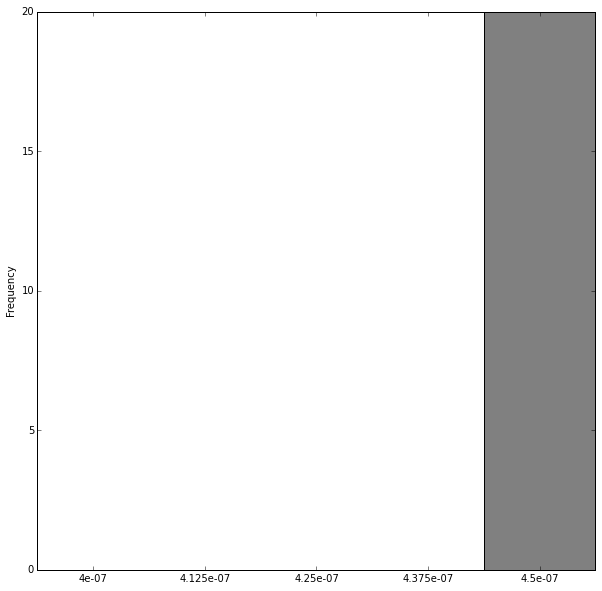
\includegraphics[scale=0.4]{hist_gd_batch_raw.png}
 \caption{Histograma}
\end{figure}

\subsubsection*{Rescaled data}
\begin{figure}[!htpb]
\centering
 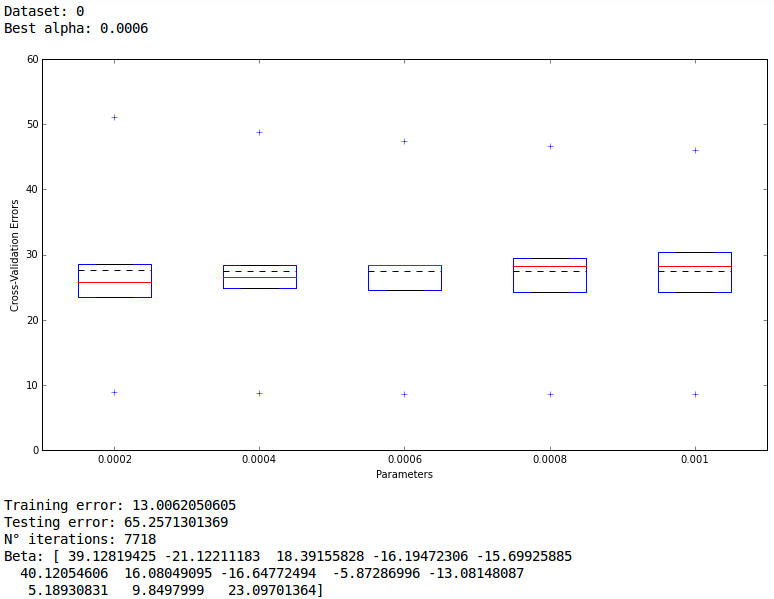
\includegraphics[scale=0.45]{gd_batch_rescaled0.png}
 \caption{Gradiente Descendente Batch - Rescaled data - dataset 0}
\end{figure}

\begin{figure}[!htpb]
\centering
 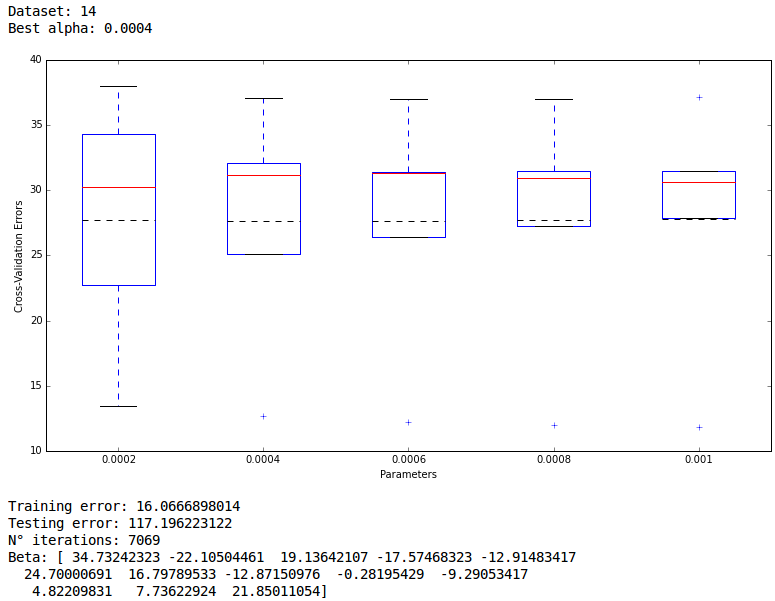
\includegraphics[scale=0.45]{gd_batch_rescaled14.png}
 \caption{Gradiente Descendente Batch - Rescaled data - dataset 14}
\end{figure}

\begin{figure}[!htpb]
\centering
 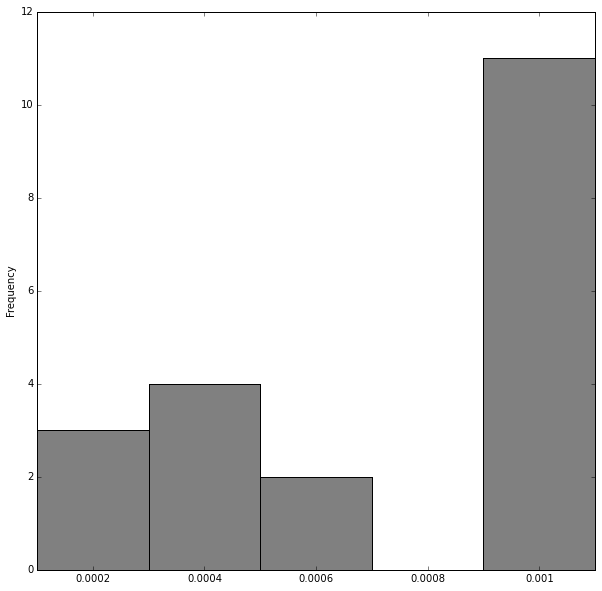
\includegraphics[scale=0.4]{hist_gd_batch_rescaled.png}
 \caption{histograma}
\end{figure}

\subsubsection*{Normalized data}
\begin{figure}[!htpb]
\centering
 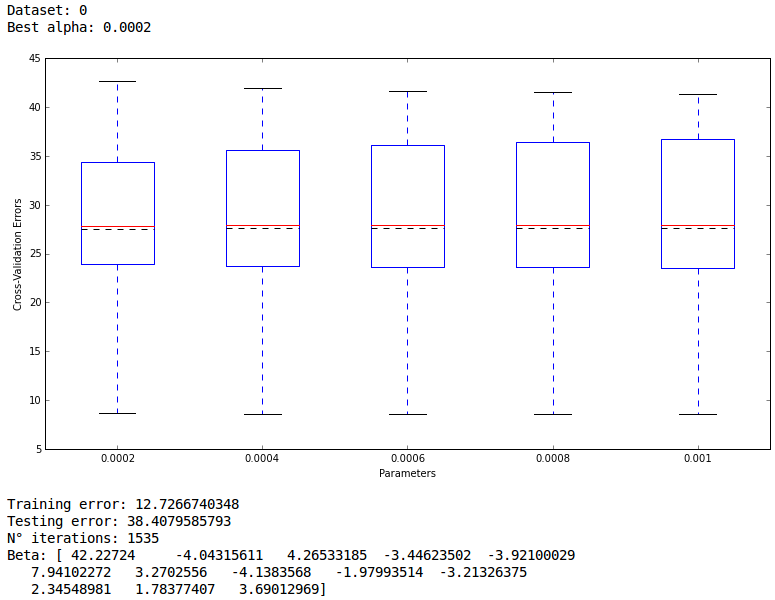
\includegraphics[scale=0.45]{gd_batch_norm0.png}
 \caption{Gradiente Descendente Batch - Normalized data - dataset 0}
\end{figure}

\begin{figure}[!htpb]
\centering
 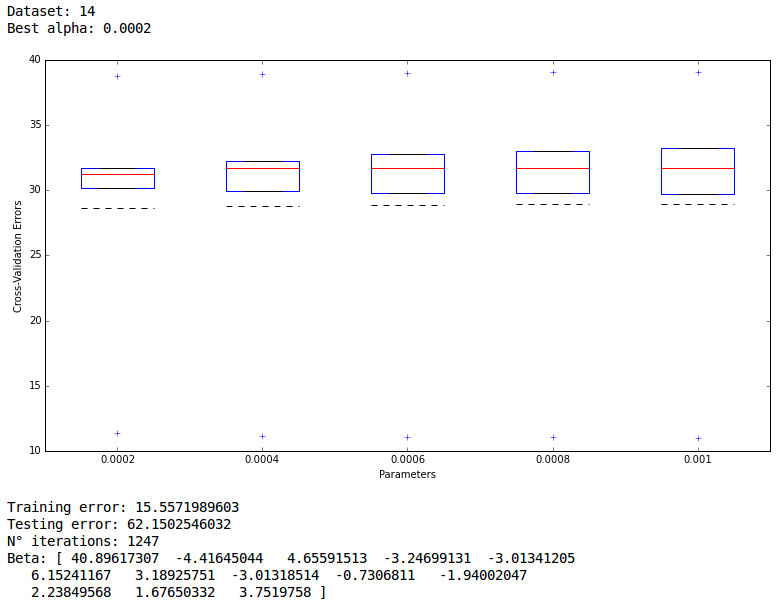
\includegraphics[scale=0.45]{gd_batch_norm14.png}
 \caption{Gradiente Descendente Batch - Normalized data - dataset 14}
\end{figure}

\begin{figure}[!htpb]
\centering
 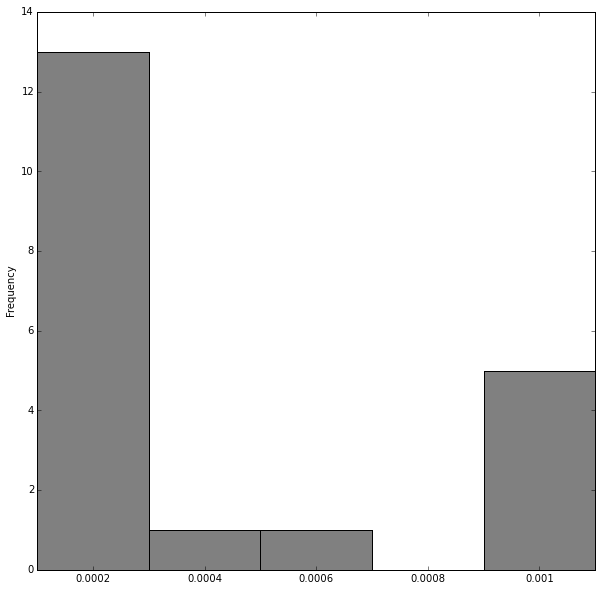
\includegraphics[scale=0.4]{hist_gd_batch_norm.png}
 \caption{Histograma}
\end{figure}






\subsection*{b) Gradiente Descendente Online}

\subsubsection*{Raw data}
\begin{figure}[!htpb]
\centering
 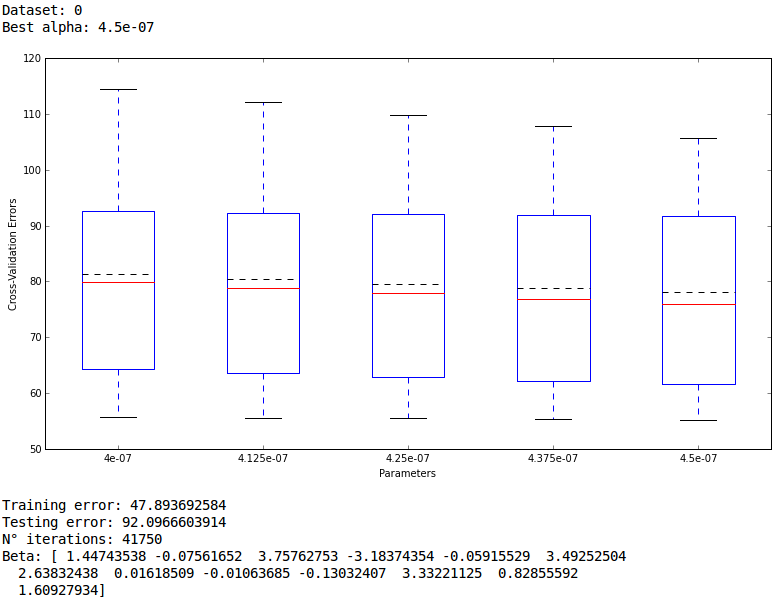
\includegraphics[scale=0.45]{gd_online_raw0.png}
 \caption{Gradiente Descendente Online - Raw data - dataset 0}
\end{figure}

\begin{figure}[!htpb]
\centering
 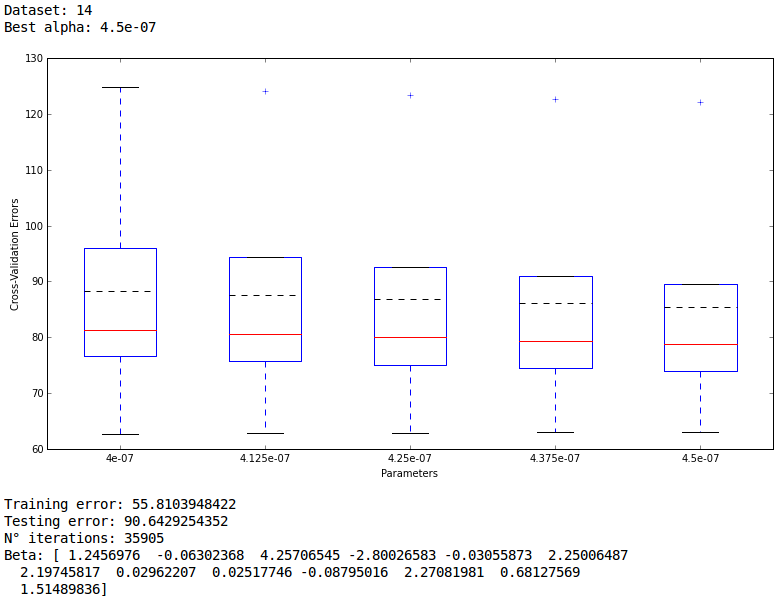
\includegraphics[scale=0.45]{gd_online_raw14.png}
 \caption{Gradiente Descendente Online - Raw data - dataset 14}
\end{figure}

\begin{figure}[!htpb]
\centering
 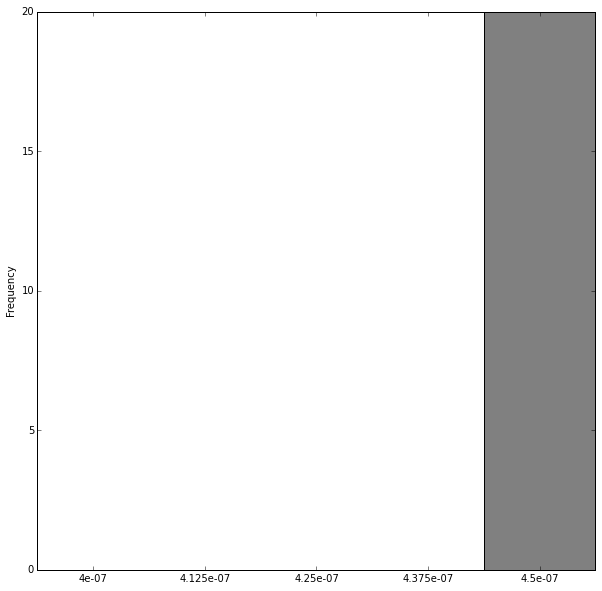
\includegraphics[scale=0.4]{hist_gd_online_raw.png}
 \caption{histograma}
\end{figure}

\subsubsection*{Rescaled data}
\begin{figure}[!htpb]
\centering
 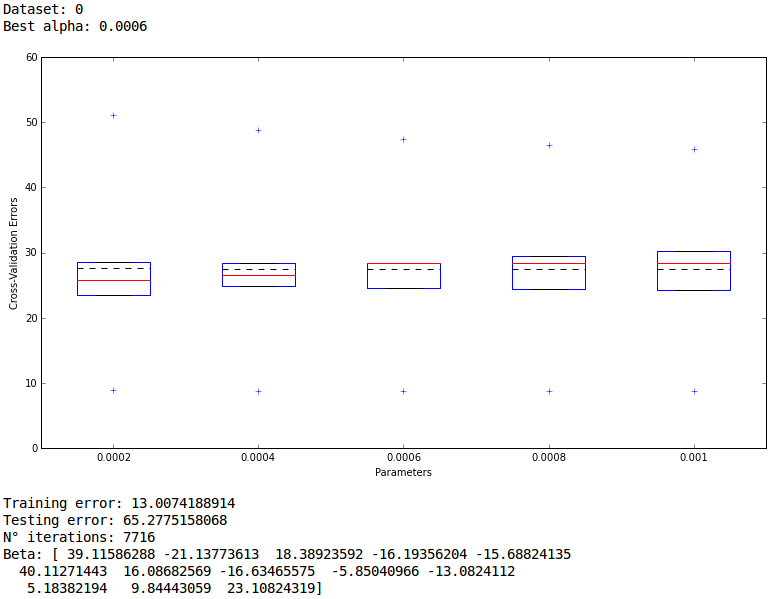
\includegraphics[scale=0.45]{gd_online_rescaled0.png}
 \caption{Gradiente Descendente Online - Rescaled data - dataset 0}
\end{figure}

\begin{figure}[!htpb]
\centering
 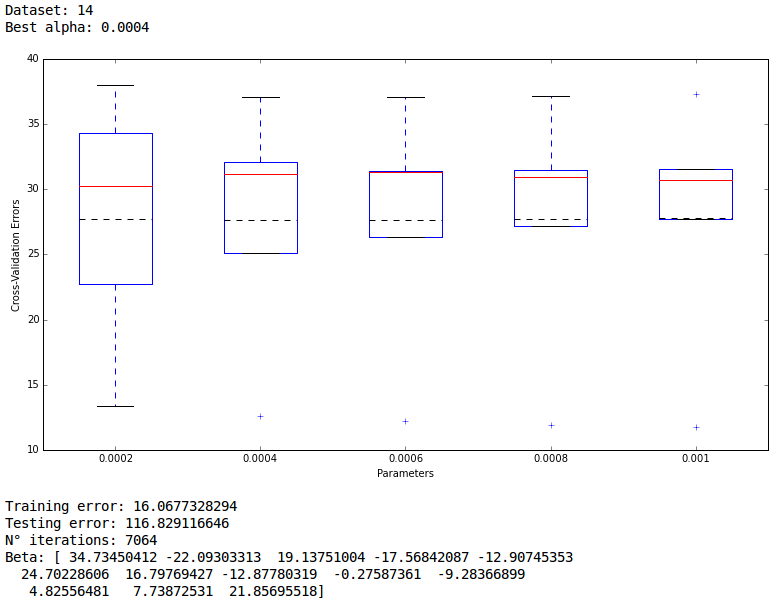
\includegraphics[scale=0.45]{gd_online_rescaled14.png}
 \caption{Gradiente Descendente Online - Rescaled data - dataset 14}
\end{figure}

\begin{figure}[!htpb]
\centering
 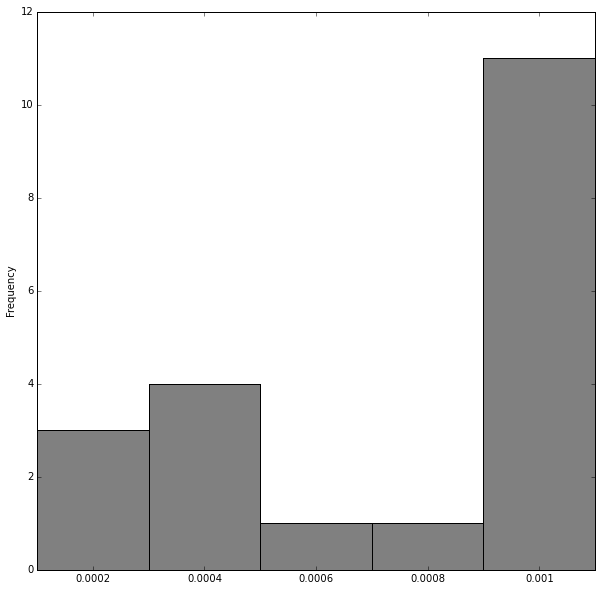
\includegraphics[scale=0.4]{hist_gd_online_rescaled.png}
 \caption{Histograma}
\end{figure}

\subsubsection*{Normalized data}
\begin{figure}[!htpb]
\centering
 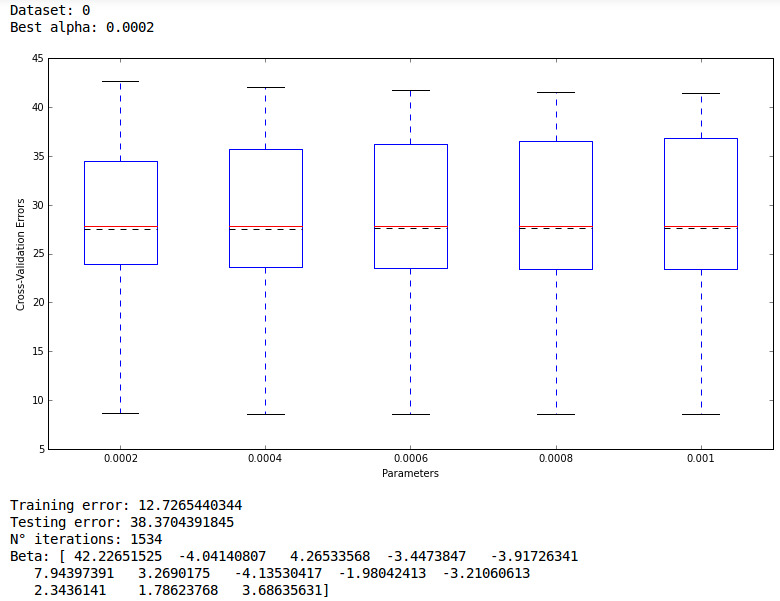
\includegraphics[scale=0.45]{gd_online_norm0.png}
 \caption{Gradiente Descendente Online - Normalized data - dataset 0}
\end{figure}

\begin{figure}[!htpb]
\centering
 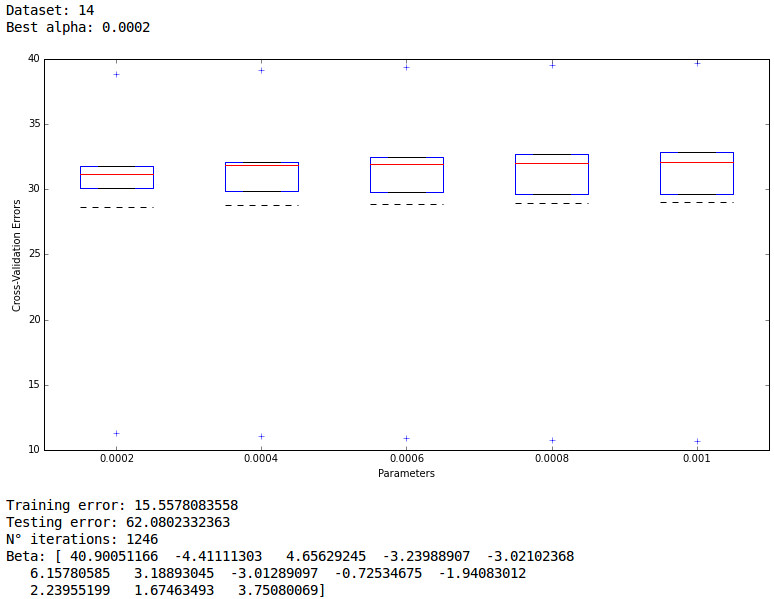
\includegraphics[scale=0.45]{gd_online_norm14.png}
 \caption{Gradiente Descendente Online - Normalized data - dataset 14}
\end{figure}

\begin{figure}[!htpb]
\centering
 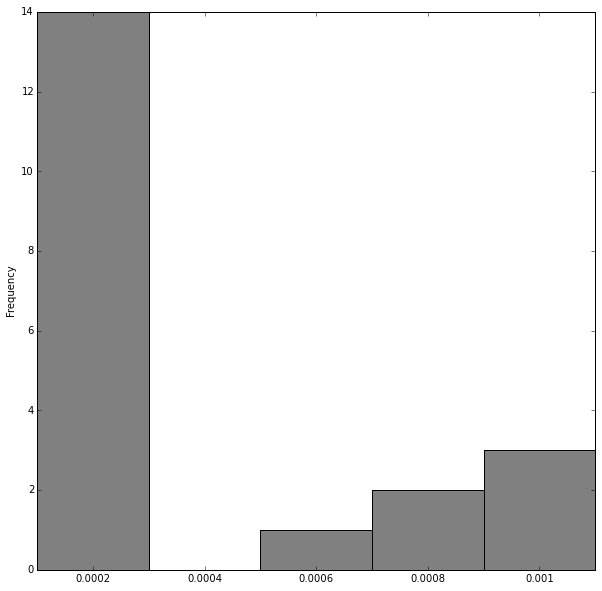
\includegraphics[scale=0.4]{hist_gd_online_norm.png}
 \caption{Histograma}
\end{figure}

\subsection{c) Newton-Raphson}

\begin{figure}[!htpb]
\centering
 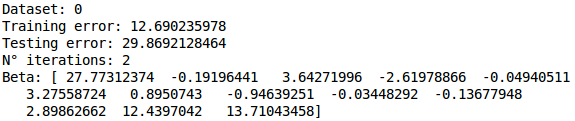
\includegraphics[scale=0.5]{nr_raw0.png}
 \caption{Newton Raphson - Raw data - dataset 0}
\end{figure}

\begin{figure}[!htpb]
\centering
 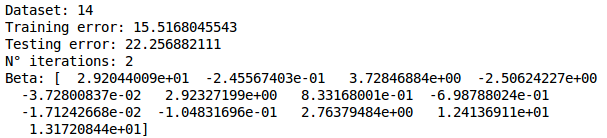
\includegraphics[scale=0.5]{nr_raw14.png}
 \caption{Newton Raphson - Raw data - dataset 14}
\end{figure}

\begin{figure}[!htpb]
\centering
 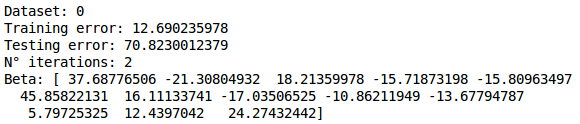
\includegraphics[scale=0.5]{nr_rescaled0.png}
 \caption{Newton Raphson - Rescaled data - dataset 0}
\end{figure}

\begin{figure}[!htpb]
\centering
 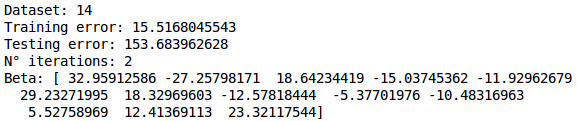
\includegraphics[scale=0.5]{nr_rescaled14.png}
 \caption{Newton Raphson - Rescaled data - dataset 14}
\end{figure}

\begin{figure}[!htpb]
\centering
 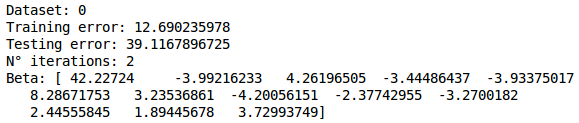
\includegraphics[scale=0.5]{nr_norm0.png}
 \caption{Newton Raphson - Normalized data - dataset 0}
\end{figure}

\begin{figure}[!htpb]
\centering
 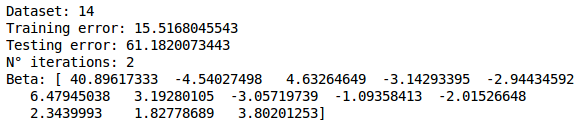
\includegraphics[scale=0.5]{nr_norm14.png}
 \caption{Newton Raphson - Normalized data - dataset 14}
\end{figure}


\begin{enumerate}
	\item 
\end{enumerate}

\item

\begin{table}[!htbp]
\centering
\begin{tabular}{|c|l|l|l|l|l|l|}
\hline
\multicolumn{1}{|l|}{\textbf{DataSet}} & \multicolumn{1}{c|}{\textbf{\begin{tabular}[c]{@{}c@{}}Training MSE\\ raw data\end{tabular}}} & \multicolumn{1}{c|}{\textbf{\begin{tabular}[c]{@{}c@{}}Training MSE\\ rescaled data\end{tabular}}} & \multicolumn{1}{c|}{\textbf{\begin{tabular}[c]{@{}c@{}}Training MSE\\ normalized data\end{tabular}}} & \multicolumn{1}{c|}{\textbf{\begin{tabular}[c]{@{}c@{}}Testing MSE\\ raw data\end{tabular}}} & \textbf{\begin{tabular}[c]{@{}l@{}}Testing MSE\\ rescaled data\end{tabular}} & \multicolumn{1}{c|}{\textbf{\begin{tabular}[c]{@{}c@{}}Testing MSE\\ normalized data\end{tabular}}} \\ \hline
0 & 47.7018651247 & 13.0062050605 & 12.7266740348 & 98.5365507026 & 65.2571301369 & 38.4079585793 \\ \hline
1 & 64.7550597054 & 16.3602257442 & 16.0715344155 & 48.2315757796 & 92.0230671423 & 65.1941175822 \\ \hline
2 & 60.7481463585 & 18.1457842322 & 17.7788520385 & 79.3615414274 & 115.610985266 & 18.2024811924 \\ \hline
3 & 58.9987667645 & 14.1017329842 & 13.9377761345 & 97.6149558458 & 171.105766665 & 48.6525469488 \\ \hline
4 & 60.3072912204 & 15.5749130727 & 15.3894271276 & 88.023192366 & 55.4477742699 & 24.1581873664 \\ \hline
5 & 50.8161360455 & 14.2610314693 & 13.3703648326 & 103.273046989 & 53.7595016258 & 27.1554482493 \\ \hline
6 & 65.6541052631 & 17.0409159049 & 15.7806050056 & 57.5892393027 & 138.507544424 & 50.1360687667 \\ \hline
7 & 55.4439862945 & 16.7780811429 & 16.5841191369 & 75.1149772436 & 47.9171960704 & 28.077556808 \\ \hline
8 & 54.5426469971 & 17.6594834655 & 17.0797580788 & 82.2107819498 & 27.7334819973 & 18.6923467845 \\ \hline
9 & 62.4168368555 & 16.3081104286 & 15.8926108555 & 59.7595593067 & 337.991435488 & 32.4322681958 \\ \hline
10 & 54.2623055884 & 13.4248859313 & 13.2809364772 & 102.249628704 & 76.0132818686 & 51.964392846 \\ \hline
11 & 62.0340545439 & 15.8168112322 & 15.1229661239 & 96.3581158257 & 29.6423010367 & 58.2778323768 \\ \hline
12 & 60.1712404807 & 14.7897334494 & 14.2704574864 & 47.6982336899 & 79.6061371602 & 33.4736955049 \\ \hline
13 & 63.8754224266 & 13.5218597059 & 13.3686890914 & 54.6855768246 & 246.084167693 & 49.4021401471 \\ \hline
14 & 55.3889121746 & 16.0666898014 & 15.5571989603 & 87.9559175097 & 117.196223122 & 62.1502546032 \\ \hline
15 & 46.1065815649 & 7.96105164535 & 7.7831599526 & 120.74160843 & 102.779537282 & 103.539701305 \\ \hline
16 & 58.7921426086 & 10.6974314356 & 10.4686233286 & 82.0169113703 & 509.388015464 & 79.8182740031 \\ \hline
17 & 65.6326333879 & 14.3023622226 & 14.0575024157 & 50.8059305089 & 72.9172185356 & 39.4462557317 \\ \hline
18 & 56.5555399322 & 16.4039458304 & 16.1738495233 & 89.5246242367 & 101.716074157 & 19.219045776 \\ \hline
19 & 53.8965499152 & 13.1956721947 & 12.7453067041 & 101.423157308 & 79.6597927613 & 41.4905102572 \\ \hline
\end{tabular}
\caption{MSE obtenidos en cada dataset con \textbf{Gradiente Descendente Batch}}
\label{my-label}
\end{table}

\begin{table}[!htbp]
\centering
\begin{tabular}{|c|l|l|l|l|l|l|}
\hline
\multicolumn{1}{|l|}{\textbf{DataSet}} & \multicolumn{1}{c|}{\textbf{\begin{tabular}[c]{@{}c@{}}Training MSE\\ raw data\end{tabular}}} & \multicolumn{1}{c|}{\textbf{\begin{tabular}[c]{@{}c@{}}Training MSE\\ rescaled data\end{tabular}}} & \multicolumn{1}{c|}{\textbf{\begin{tabular}[c]{@{}c@{}}Training MSE\\ normalized data\end{tabular}}} & \multicolumn{1}{c|}{\textbf{\begin{tabular}[c]{@{}c@{}}Testing MSE\\ raw data\end{tabular}}} & \textbf{\begin{tabular}[c]{@{}l@{}}Testing MSE\\ rescaled data\end{tabular}} & \multicolumn{1}{c|}{\textbf{\begin{tabular}[c]{@{}c@{}}Testing MSE\\ normalized data\end{tabular}}} \\ \hline
0  & 47.893692584 & 13.0074188914 & 12.7265440344 & 92.0966603914 & 65.2775158068 & 38.3704391845 \\ \hline
1  & 64.6988609429 & 16.3629180412 & 16.0711580478 & 47.9123694862 & 93.6913520605 & 65.2908059333 \\ \hline
2  & 60.9392772213 & 18.1476046506 & 17.7880949034 & 78.1358655876 & 115.411791641 & 18.0041725612 \\ \hline
3  & 58.9787768796 & 14.1002166575 & 13.9375577433 & 99.2667062665 & 171.566596167 & 48.6369000543 \\ \hline
4  & 60.1774212144 & 15.5749021184 & 15.3892917875 & 88.333392035 & 55.4869693485 & 24.1745417821 \\ \hline
5  & 51.0422341216 & 14.260531204 & 13.370563385 & 103.788709289 & 53.7282011004 & 27.1142854438 \\ \hline
6  & 65.5165575721 & 17.0406053124 & 15.7815019554 & 57.4194579169 & 138.43489681 & 50.2731709417 \\ \hline
7  & 55.3588268682 & 16.780307963 & 16.5841646531 & 75.6410018834 & 47.5944048007 & 28.0681605601 \\ \hline
8  & 54.6439352519 & 17.6584519859 & 17.0797739827 & 80.7421944912 & 27.7337192325 & 18.6695277152 \\ \hline
9  & 62.1799637644 & 16.1913895977 & 15.892886139 & 58.8581361381 & 342.077775481 & 32.407908827 \\ \hline
10 & 54.2693780177 & 13.4256912568 & 13.2804573566 & 102.231247534 & 75.9971396011 & 52.0015285506 \\ \hline
11 & 62.2595665841 & 15.8160994494 & 15.1230550605 & 86.3623966795 & 29.6439787773 & 58.2777057111 \\ \hline
12 & 60.2843606249 & 14.7899074557 & 14.2703041781 & 48.357913035 & 79.7909631268 & 33.5181606162 \\ \hline
13 & 63.2651920301 & 13.5241617939 & 13.3663998961 & 53.681043548 & 245.88695962 & 49.3798234136 \\ \hline
14 & 55.8103948422 & 16.0677328294 & 15.5578083558 & 90.6429254352 & 116.829116646 & 62.0802332363 \\ \hline
15 & 45.8872186824 & 7.96097566712 & 7.7830831329 & 120.024573066 & 102.830744793 & 103.525379024 \\ \hline
16 & 59.139425774 & 10.700077422 & 10.4703925557 & 84.7003440117 & 507.801818338 & 80.0407382824 \\ \hline
17 & 65.8135992766 & 14.3060025597 & 14.0814594646 & 51.1345452402 & 73.3125213211 & 39.0982468252 \\ \hline
18 & 56.780939942 & 16.4046917857 & 16.1771940462 & 89.4773158001 & 100.697687488 & 19.2541349743 \\ \hline
19 & 56.4175529102 & 13.1946751264 & 12.74837702 & 95.239291694 & 79.7129789852 & 41.4471018701 \\ \hline
\end{tabular}
\caption{MSE obtenidos en cada dataset con \textbf{Gradiente Descendente Online}}
\label{my-label}
\end{table}


\begin{table}[!htbp]
\centering
\begin{tabular}{|c|l|l|l|l|l|l|}
\hline
\multicolumn{1}{|l|}{\textbf{DataSet}} & \multicolumn{1}{c|}{\textbf{\begin{tabular}[c]{@{}c@{}}Training MSE\\ raw data\end{tabular}}} & \multicolumn{1}{c|}{\textbf{\begin{tabular}[c]{@{}c@{}}Training MSE\\ rescaled data\end{tabular}}} & \multicolumn{1}{c|}{\textbf{\begin{tabular}[c]{@{}c@{}}Training MSE\\ normalized data\end{tabular}}} & \multicolumn{1}{c|}{\textbf{\begin{tabular}[c]{@{}c@{}}Testing MSE\\ raw data\end{tabular}}} & \textbf{\begin{tabular}[c]{@{}l@{}}Testing MSE\\ rescaled data\end{tabular}} & \multicolumn{1}{c|}{\textbf{\begin{tabular}[c]{@{}c@{}}Testing MSE\\ normalized data\end{tabular}}} \\ \hline
0  & 12.690235978 & 12.690235978 & 12.690235978 & 29.8692128464 & 70.8230012379 & 39.1167896725 \\ \hline
1  & 15.9947888908 & 15.9947888908 & 15.9947888908 & 19.1213963039 & 105.300112485 & 67.378076989 \\ \hline
2  & 17.7637059001 & 17.7637059001 & 17.7637059001 & 13.1702299683 & 139.177707921 & 18.9190672901 \\ \hline
3  & 13.9043524941 & 13.9043524941 & 13.9043524941 & 28.1945882457 & 191.26333343 & 49.6104454505 \\ \hline
4  & 15.3443534674 & 15.3443534674 & 15.3443534674 & 18.5845078343 & 60.566792667 & 24.2427186032 \\ \hline
5  & 13.3367816832 & 13.3367816832 & 13.3367816832 & 29.3915243362 & 58.7330478202 & 26.930481888 \\ \hline
6  & 15.7714352077 & 15.7714352077 & 15.7714352077 & 19.0828661051 & 183.563542547 & 50.2499676832 \\ \hline
7  & 16.5377588238 & 16.5377588238 & 16.5377588238 & 16.3703204049 & 50.4205344035 & 28.4870497309 \\ \hline
8  & 17.0315091906 & 17.0315091906 & 17.0315091906 & 16.1490495786 & 30.3017645531 & 18.8447579043 \\ \hline
9  & 15.8241747153 & 15.8241747153 & 15.8241747153 & 21.9579912403 & 363.7143535 & 34.6682484071 \\ \hline
10 & 13.2459812442 & 13.2459812442 & 13.2459812442 & 31.6607303987 & 77.7453577289 & 51.7167752009 \\ \hline
11 & 15.0861602358 & 15.0861602358 & 15.0861602358 & 30.0689055712 & 30.5014191423 & 57.8116748334 \\ \hline
12 & 14.2247910054 & 14.2247910054 & 14.2247910054 & 29.1616123114 & 85.4768097109 & 33.1587602379 \\ \hline
13 & 13.3574116939 & 13.3574116939 & 13.3574116939 & 29.9555390274 & 245.72965064 & 49.7847446069 \\ \hline
14 & 15.5168045543 & 15.5168045543 & 15.5168045543 & 22.256882111 & 153.683962628 & 61.1820073443 \\ \hline
15 & 7.74295071369 & 7.74295071369 & 7.74295071369 & 86.5926285733 & 119.511903868 & 108.660106191 \\ \hline
16 & 10.4584851241 & 10.4584851241 & 10.4584851241 & 40.2690867836 & 609.941477727 & 81.8616628828 \\ \hline
17 & 14.0324636777 & 14.0324636777 & 14.0324636777 & 27.1971535112 & 76.3009933269 & 40.5837491905 \\ \hline
18 & 16.1663277544 & 16.1663277544 & 16.1663277544 & 18.400069049 & 120.393356486 & 19.3481384185 \\ \hline
19 & 12.7383399098 & 12.7383399098 & 12.7383399098 & 30.4741332593 & 90.2870113388 & 41.4018142274 \\ \hline
\end{tabular}
\caption{MSE obtenidos en cada dataset con \textbf{Newton Raphson}}
\label{my-label}
\end{table}


\item 

\begin{table}[!htbp]
\centering
\begin{tabular}{|c|l|l|l|l|l|l|}
\hline
\multicolumn{1}{|l|}{\textbf{DataSet}} & \multicolumn{1}{c|}{\textbf{\begin{tabular}[c]{@{}c@{}}Mean MSE (tr)\\ raw data\end{tabular}}} & \multicolumn{1}{c|}{\textbf{\begin{tabular}[c]{@{}c@{}}Mean MSE (tr)\\ rescaled data\end{tabular}}} & \multicolumn{1}{c|}{\textbf{\begin{tabular}[c]{@{}c@{}}Mean MSE (tr) \\ normalized data\end{tabular}}} & \multicolumn{1}{c|}{\textbf{\begin{tabular}[c]{@{}c@{}}Mean MSE (ts)\\ raw data\end{tabular}}} & \textbf{\begin{tabular}[c]{@{}l@{}}Mean MSE (ts) \\ rescaled data\end{tabular}} & \multicolumn{1}{c|}{\textbf{\begin{tabular}[c]{@{}c@{}}Mean MSE (ts)\\ normalized data\end{tabular}}} \\ \hline
0  & 13.9708194542 & 12.8680336262 & 14.0754337259 & 30.6070325793 & 70.2538422886 & 38.1545878007 \\ \hline
1  & 18.0834806163 & 16.3143264633 & 17.7223930193 & 22.6550523419 & 99.1910099095 & 66.6584495258 \\ \hline
2  & 21.4196770173 & 18.0574200441 & 19.7083569141 & 17.7138988198 & 135.658713423 & 17.4309022828 \\ \hline
3  & 16.8567971204 & 13.9284868171 & 15.8124146734 & 32.0918273124 & 190.57869645 & 49.5329486555 \\ \hline
4  & 18.0078316461 & 15.3822857197 & 16.9837941852 & 20.8119059567 & 61.2827227799 & 26.8131400608 \\ \hline
5  & 14.9922793796 & 15.200730076 & 14.8109358791 & 31.7423982776 & 59.0498559417 & 29.5464336581 \\ \hline
6  & 18.4642742127 & 16.0807912238 & 18.0039098954 & 20.4255284121 & 174.708314609 & 47.9711074794 \\ \hline
7  & 19.7024131836 & 16.5644574215 & 18.1680024605 & 17.9886674822 & 50.1065481925 & 25.1853276102 \\ \hline
8  & 19.4248121369 & 17.0665068591 & 19.3958302116 & 20.3804601741 & 30.8334644696 & 21.255460018 \\ \hline
9  & 17.9357297991 & 15.9039272911 & 17.3763644859 & 24.1172864169 & 362.087098812 & 36.1468796687 \\ \hline
10 & 15.7386860524 & 13.2708088805 & 15.0306952387 & 33.3096588712 & 76.8828416336 & 50.6454977071 \\ \hline
11 & 17.3194968818 & 15.1099160935 & 16.4193094944 & 28.9740381478 & 30.4467078354 & 56.3551072141 \\ \hline
12 & 16.0366659073 & 14.2436358884 & 15.1784417823 & 28.3158666633 & 85.4381137078 & 35.2075508589 \\ \hline
13 & 15.2138849104 & 13.3810755139 & 14.7671579436 & 30.5263839969 & 243.810200428 & 45.8707565488 \\ \hline
14 & 17.9772193096 & 15.8910639207 & 17.9931698801 & 28.8310546838 & 158.00874091 & 62.4797627491 \\ \hline
15 & 9.4699799064 & 7.78945051406 & 8.80284013072 & 97.3248544308 & 119.235710082 & 108.999763541 \\ \hline
16 & 12.0919856379 & 10.6807108655 & 11.578698134 & 44.094575934 & 587.161557697 & 78.6737437855 \\ \hline
17 & 16.0292750664 & 14.0616360113 & 16.4744564074 & 34.4008235114 & 74.3334497261 & 39.0643258942 \\ \hline
18 & 18.6281507772 & 16.4797651978 & 18.2085555161 & 22.0902895146 & 120.787437358 & 18.80628939 \\ \hline
19 & 14.7544905309 & 13.0303465155 & 13.9650302619 & 31.2766943345 & 89.005555994 & 44.4494974151 \\ \hline
\end{tabular}
\caption{Mean MSE en cada dataset con \textbf{Locally Weighted Linear Regression}}
\label{my-label}
\end{table}





\end{enumerate}



\newpage
\section*{Parte 2- Regresión Logística}

\begin{enumerate}
 \item asdf

 \item qwerty

\begin{table}[!htbp]
\centering
\begin{tabular}{|c|l|l|l|l|l|l|}
\hline
\multicolumn{1}{|l|}{\textbf{DataSet}} & \multicolumn{1}{c|}{\textbf{\begin{tabular}[c]{@{}c@{}}Error rate (tr)\\ raw data\end{tabular}}} & \multicolumn{1}{c|}{\textbf{\begin{tabular}[c]{@{}c@{}}Error rate (tr)\\ rescaled data\end{tabular}}} & \multicolumn{1}{c|}{\textbf{\begin{tabular}[c]{@{}c@{}}Error rate (tr)\\ normalized data\end{tabular}}} & \multicolumn{1}{c|}{\textbf{\begin{tabular}[c]{@{}c@{}}Error rate (ts)\\ raw data\end{tabular}}} & \textbf{\begin{tabular}[c]{@{}l@{}}Error rate (ts)\\ rescaled data\end{tabular}} & \multicolumn{1}{c|}{\textbf{\begin{tabular}[c]{@{}c@{}}Error rate (ts)\\ normalized data\end{tabular}}} \\ \hline
0  & 0.0444444444444 & 0.0666666666667 & 0.0222222222222 & 0.0666666666667 & 0.1 & 0.0333333333333 \\ \hline
1  & 0.0444444444444 & 0.0555555555556 & 0.0444444444444 & 0.0333333333333 & 0.0 & 0.1 \\ \hline
2  & 0.266666666667 & 0.0444444444444 & 0.0222222222222 & 0.333333333333 & 0.3 & 0.133333333333 \\ \hline
3  & 0.0666666666667 & 0.0555555555556 & 0.0222222222222 & 0.0333333333333 & 0.166666666667 & 0.0666666666667 \\ \hline
4  & 0.0666666666667 & 0.0777777777778 & 0.0444444444444 & 0.1 & 0.0333333333333 & 0.166666666667 \\ \hline
5  & 0.188888888889 & 0.0777777777778 & 0.0333333333333 & 0.166666666667 & 0.0333333333333 & 0.0333333333333 \\ \hline
6  & 0.0777777777778 & 0.0555555555556 & 0.0222222222222 & 0.233333333333 & 0.1 & 0.0333333333333 \\ \hline
7  & 0.177777777778 & 0.0888888888889 & 0.0666666666667 & 0.0 & 0.0666666666667 & 0.0666666666667 \\ \hline
8  & 0.188888888889 & 0.0444444444444 & 0.0222222222222 & 0.133333333333 & 0.0666666666667 & 0.1 \\ \hline
9  & 0.155555555556 & 0.0777777777778 & 0.0444444444444 & 0.0666666666667 & 0.1 & 0.0666666666667 \\ \hline
10 & 0.111111111111 & 0.0666666666667 & 0.0333333333333 & 0.166666666667 & 0.1 & 0.0666666666667 \\ \hline
11 & 0.0444444444444 & 0.0666666666667 & 0.0333333333333 & 0.0666666666667 & 0.133333333333 & 0.0666666666667 \\ \hline
12 & 0.2 & 0.0777777777778 & 0.0555555555556 & 0.133333333333 & 0.133333333333 & 0.0 \\ \hline
13 & 0.277777777778 & 0.0555555555556 & 0.0555555555556 & 0.366666666667 & 0.1 & 0.1 \\ \hline
14 & 0.155555555556 & 0.0888888888889 & 0.0444444444444 & 0.166666666667 & 0.1 & 0.0666666666667 \\ \hline
15 & 0.144444444444 & 0.0777777777778 & 0.0333333333333 & 0.0666666666667 & 0.0666666666667 & 0.0666666666667 \\ \hline
16 & 0.0444444444444 & 0.0333333333333 & 0.0333333333333 & 0.133333333333 & 0.0666666666667 & 0.133333333333 \\ \hline
17 & 0.0555555555556 & 0.0666666666667 & 0.0333333333333 & 0.0666666666667 & 0.0333333333333 & 0.133333333333 \\ \hline
18 & 0.0222222222222 & 0.0777777777778 & 0.0222222222222 & 0.1 & 0.133333333333 & 0.0333333333333 \\ \hline
19 & 0.188888888889 & 0.0444444444444 & 0.0111111111111 & 0.266666666667 & 0.2 & 0.133333333333 \\ \hline
\end{tabular}
\caption{Error rate en cada dataset obtenido con \textbf{Gradiente Ascendente Online} para regresión logística}
\label{my-label}
\end{table}

\begin{table}[!htbp]
\centering
\begin{tabular}{|c|l|l|l|l|l|l|}
\hline
\multicolumn{1}{|l|}{\textbf{DataSet}} & \multicolumn{1}{c|}{\textbf{\begin{tabular}[c]{@{}c@{}}Error rate (tr)\\ raw data\end{tabular}}} & \multicolumn{1}{c|}{\textbf{\begin{tabular}[c]{@{}c@{}}Error rate (tr)\\ rescaled data\end{tabular}}} & \multicolumn{1}{c|}{\textbf{\begin{tabular}[c]{@{}c@{}}Error rate (tr)\\ normalized data\end{tabular}}} & \multicolumn{1}{c|}{\textbf{\begin{tabular}[c]{@{}c@{}}Error rate (ts)\\ raw data\end{tabular}}} & \textbf{\begin{tabular}[c]{@{}l@{}}Error rate (ts)\\ rescaled data\end{tabular}} & \multicolumn{1}{c|}{\textbf{\begin{tabular}[c]{@{}c@{}}Error rate (ts)\\ normalized data\end{tabular}}} \\ \hline
0  & 0.0 & 0.0 & 0.0 & 0.0666666666667 & 0.1 & 0.0333333333333 \\ \hline
1  & 0.0 & 0.0 & 0.0 & 0.0666666666667 & 0.0666666666667 & 0.0666666666667 \\ \hline
2  & 0.0 & 0.0 & 0.0 & 0.1 & 0.2 & 0.133333333333 \\ \hline
3  & 0.0 & 0.0 & 0.0 & 0.0666666666667 & 0.166666666667 & 0.0666666666667 \\ \hline
4  & 0.0 & 0.0 & 0.0 & 0.0666666666667 & 0.0666666666667 & 0.166666666667 \\ \hline
5  & 0.0 & 0.0 & 0.0 & 0.0333333333333 & 0.0333333333333 & 0.0666666666667 \\ \hline
6  & 0.0 & 0.0 & 0.0 & 0.133333333333 & 0.133333333333 & 0.0333333333333 \\ \hline
7  & 0.0222222222222 & 0.0222222222222 & 0.0222222222222 & 0.0333333333333 & 0.0333333333333 & 0.0333333333333 \\ \hline
8  & 0.0 & 0.0 & 0.0 & 0.0666666666667 & 0.0666666666667 & 0.0666666666667 \\ \hline
9  & 0.755555555556 & 0.866666666667 & 0.622222222222 & 0.833333333333 & 0.666666666667 & 0.533333333333 \\ \hline
10 & 0.0 & 0.0 & 0.0 & 0.0666666666667 & 0.1 & 0.1 \\ \hline
11 & 0.1 & 0.133333333333 & 0.633333333333 & 0.133333333333 & 0.233333333333 & 0.4 \\ \hline
12 & 0.0 & 0.0 & 0.0 & 0.0333333333333 & 0.0333333333333 & 0.0333333333333 \\ \hline
13 & 0.522222222222 & 0.588888888889 & 0.6 & 0.566666666667 & 0.733333333333 & 0.633333333333 \\ \hline
14 & 0.111111111111 & 0.788888888889 & 0.455555555556 & 0.0333333333333 & 0.566666666667 & 0.733333333333 \\ \hline
15 & 0.0222222222222 & 0.0222222222222 & 0.4 & 0.0666666666667 & 0.166666666667 & 0.333333333333 \\ \hline
16 & 0.0 & 0.0 & 0.0 & 0.166666666667 & 0.166666666667 & 0.2  \\ \hline
17 & 0.0 & 0.0 & 0.0 & 0.0666666666667 & 0.166666666667 & 0.133333333333 \\ \hline
18 & 0.0 & 0.0 & 0.0 & 0.0666666666667 & 0.0333333333333 & 0.1 \\ \hline
19 & 0.0 & 0.0 & 0.0 & 0.133333333333 & 0.133333333333 & 0.133333333333\\ \hline
\end{tabular}
\caption{Error rate en cada dataset obtenido con \textbf{Newton Raphson} para regresión logística}
\label{my-label}
\end{table}

 \item asdf
\end{enumerate}

\newpage
\section*{Anexo}

\subsection*{Implementación de algoritmos para regresión lineal}

\begin{python}
def gd_batch(X, y, alpha, eps=1e-5, max_iter=100000):
    M,N = X.shape
    beta = np.zeros(N)
    J1 = J(X,y,beta)
    for i in xrange(max_iter):
        J0 = J1
        f = np.dot(X,beta)
        dJ = np.dot(X.T,f-y)
        beta -= alpha*dJ
        J1 = J(X,y,beta)
        if np.abs(J1-J0)/J0 < eps:
            break
    return (beta,i+1)
\end{python}

\begin{python}
def gd_online(X, y, alpha, eps=1e-5, max_iter=100000):
    M,N = X.shape
    beta = np.zeros(N)
    J1 = J(X,y,beta)
    for i in xrange(max_iter):
        J0 = J1
        for m in xrange(M):
            beta -= alpha*(np.dot(X[m],beta)-y[m])*X[m]
        J1 = J(X,y,beta)
        if np.abs(J1-J0)/J0 < eps: break
    return (beta,i+1)
\end{python}

\begin{python}
def nr_linear(X, y, eps=1e-5, max_iter=100000):
    M,N = X.shape
    beta = np.zeros(N)
    J1 = J(X,y,beta)
    Hess = np.dot(X.T,X)
    for i in xrange(max_iter):
        J0 = J1
        f = np.dot(X,beta)
        dJ = np.dot(X.T,f-y)
        beta -= np.linalg.solve(Hess, dJ)
        J1 = J(X,y,beta)
        if np.abs(J1-J0)/J0 < eps: break
    return (beta,i+1)
\end{python}

\subsubsection*{Comentarios de implementación}
\begin{enumerate}
	\item Para todos los algoritmos existen básicamente dos criterios de salida. El primero es
	cuando el error relativo es menor a \texttt{eps}, vale decir, cuando la función de error esta
	cambiando muy poco de iteración en iteración. El segundo es el número máximo de iteraciones, mas
	que nada para detener algoritmos que no pueden cumplir con el criterio del error (learning rates muy
	altos por ejemplo).
	\item Todos los \textit{starting guest} son el vector zeros. Esto para reproducir y comparar resultados
	de manera adecuada.
	\item En vez de invertir la matriz Hessiana en Newton-Raphson, se opta por resolver el sistema lineal
	asociado, por razones de estabilidad numérica.
\end{enumerate}

\newpage
\subsection*{Implementación de algoritmos para regresión logística}

\begin{python}
def gd_stochastic(X, y, alpha, eps=1e-3, max_iter=100000):
    M,N = X.shape
    beta = np.zeros(N)
    l1 = l(X, y, beta)+1.
    for i in xrange(max_iter):
        l0 = l1
        for m in xrange(M):
            beta += alpha*(y[m]-sigmoid(np.dot(X[m],beta)))*X[m]
        l1 = l(X,y,beta)+1.
        if np.abs(l1-l0)/np.abs(l0) < eps: break
    return (beta,i+1)
\end{python}

\begin{python}
def nr_logistic(X, y, alpha, eps=1e-3, max_iter=100000):
    M,N = X.shape
    beta = np.zeros(N)
    l1 = l(X, y, beta)+1.
    for i in xrange(max_iter):
        l0 = l1
        f = sigmoid(np.dot(X,beta))
        W = np.diag(f*(1-f))
        Hess = -1*np.dot(X.T, np.dot(W, X))
        Dl = np.dot(X.T, y-f)
        try:
            beta -= alpha*np.linalg.solve(Hess, Dl)
        except np.linalg.LinAlgError:
            break
        l1 = l(X, y, beta)+1.
        if np.abs(l1-l0)/np.abs(l0) < eps: break
    return (beta,i+1)
\end{python}

\subsubsection*{Comentarios de implementación}
\begin{enumerate}
	\item Para ambos algoritmos hay dos criterios de salida. El primero es cuando la función \textit{log verosimilitud} cambia relativamente menor a \texttt{eps} en cada iteración (pues es la función que se quiere maximizar). Se tiene en cuenta además que en el óptimo esta función debe ser $0$ (en el óptimo la función de \textit{verosimilitud} es $1$, pues maximiza la probabilidad para cada dato), por lo que se le suma un $1$ para evitar problemas al computar el criterio de salida. El segundo criterio el número máximo de iteraciones.
	\item Existe un tercer criterio de salida en el método de \textit{Newton-Raphson}. A medida que converge, el vector $f$ con las probabilidades de pertenecer a la clase $1$ de todos los datos, tiene sólo valores cercanos a $0$ y $1$. Luego al computar la matriz $W$, esta empezará a tener filas completas de $0$ o valores muy cercanos a $0$, y por lo tanto la matriz Hessiana también, y al converger esta matriz se vuelve singular. Para eso se ocupa el manejo de la excepción en caso de existir singularidad.

\end{enumerate}

\vfill\hfill MV/\LaTeXe
\end{document}



% \begin{table}[!htbp]
% \centering
% \begin{tabular}{|c|l|l|l|l|l|l|}
% \hline
% \multicolumn{1}{|l|}{\textbf{DataSet}} & \multicolumn{1}{c|}{\textbf{\begin{tabular}[c]{@{}c@{}}Training MSE\\ raw data\end{tabular}}} & \multicolumn{1}{c|}{\textbf{\begin{tabular}[c]{@{}c@{}}Training MSE\\ rescaled data\end{tabular}}} & \multicolumn{1}{c|}{\textbf{\begin{tabular}[c]{@{}c@{}}Training MSE\\ normalized data\end{tabular}}} & \multicolumn{1}{c|}{\textbf{\begin{tabular}[c]{@{}c@{}}Testing MSE\\ raw data\end{tabular}}} & \textbf{\begin{tabular}[c]{@{}l@{}}Testing MSE\\ rescaled data\end{tabular}} & \multicolumn{1}{c|}{\textbf{\begin{tabular}[c]{@{}c@{}}Testing MSE\\ normalized data\end{tabular}}} \\ \hline
% 0 &  &  &  &  &  &  \\ \hline
% 1 &  &  &  &  &  &  \\ \hline
% 2 &  &  &  &  &  &  \\ \hline
% 3 &  &  &  &  &  &  \\ \hline
% 4 &  &  &  &  &  &  \\ \hline
% 5 &  &  &  &  &  &  \\ \hline
% 6 &  &  &  &  &  &  \\ \hline
% 7 &  &  &  &  &  &  \\ \hline
% 8 &  &  &  &  &  &  \\ \hline
% 9 &  &  &  &  &  &  \\ \hline
% 10 &  &  &  &  &  &  \\ \hline
% 11 &  &  &  &  &  &  \\ \hline
% 12 &  &  &  &  &  &  \\ \hline
% 13 &  &  &  &  &  &  \\ \hline
% 14 &  &  &  &  &  &  \\ \hline
% 15 &  &  &  &  &  &  \\ \hline
% 16 &  &  &  &  &  &  \\ \hline
% 17 &  &  &  &  &  &  \\ \hline
% 18 &  &  &  &  &  &  \\ \hline
% 19 &  &  &  &  &  &  \\ \hline
% \end{tabular}
% \caption{MSE de modelo con Gradiente Descendente Batch sobre dataset}
% \label{my-label}
% \end{table}
